%!TeX root=../main.tex

\chapter{Desenvolvimento}
\label{cap:desenvolvimento}

    O sistema do Shogi-sensei pode ser dividido em quatro blocos principais: o banco de dados, a \textit{engine} do YaneuraOu, o servidor e por fim a interface. A relação entre esses componentes é apresentada na Figura~\ref{fig:system_overview}. Cada bloco foi desenvolvido em um \textit{docker container} diferente, com o intuito de permitir que o projeto possa ser executado em qualquer máquina.

    \begin{figure}[H]
        \centering
        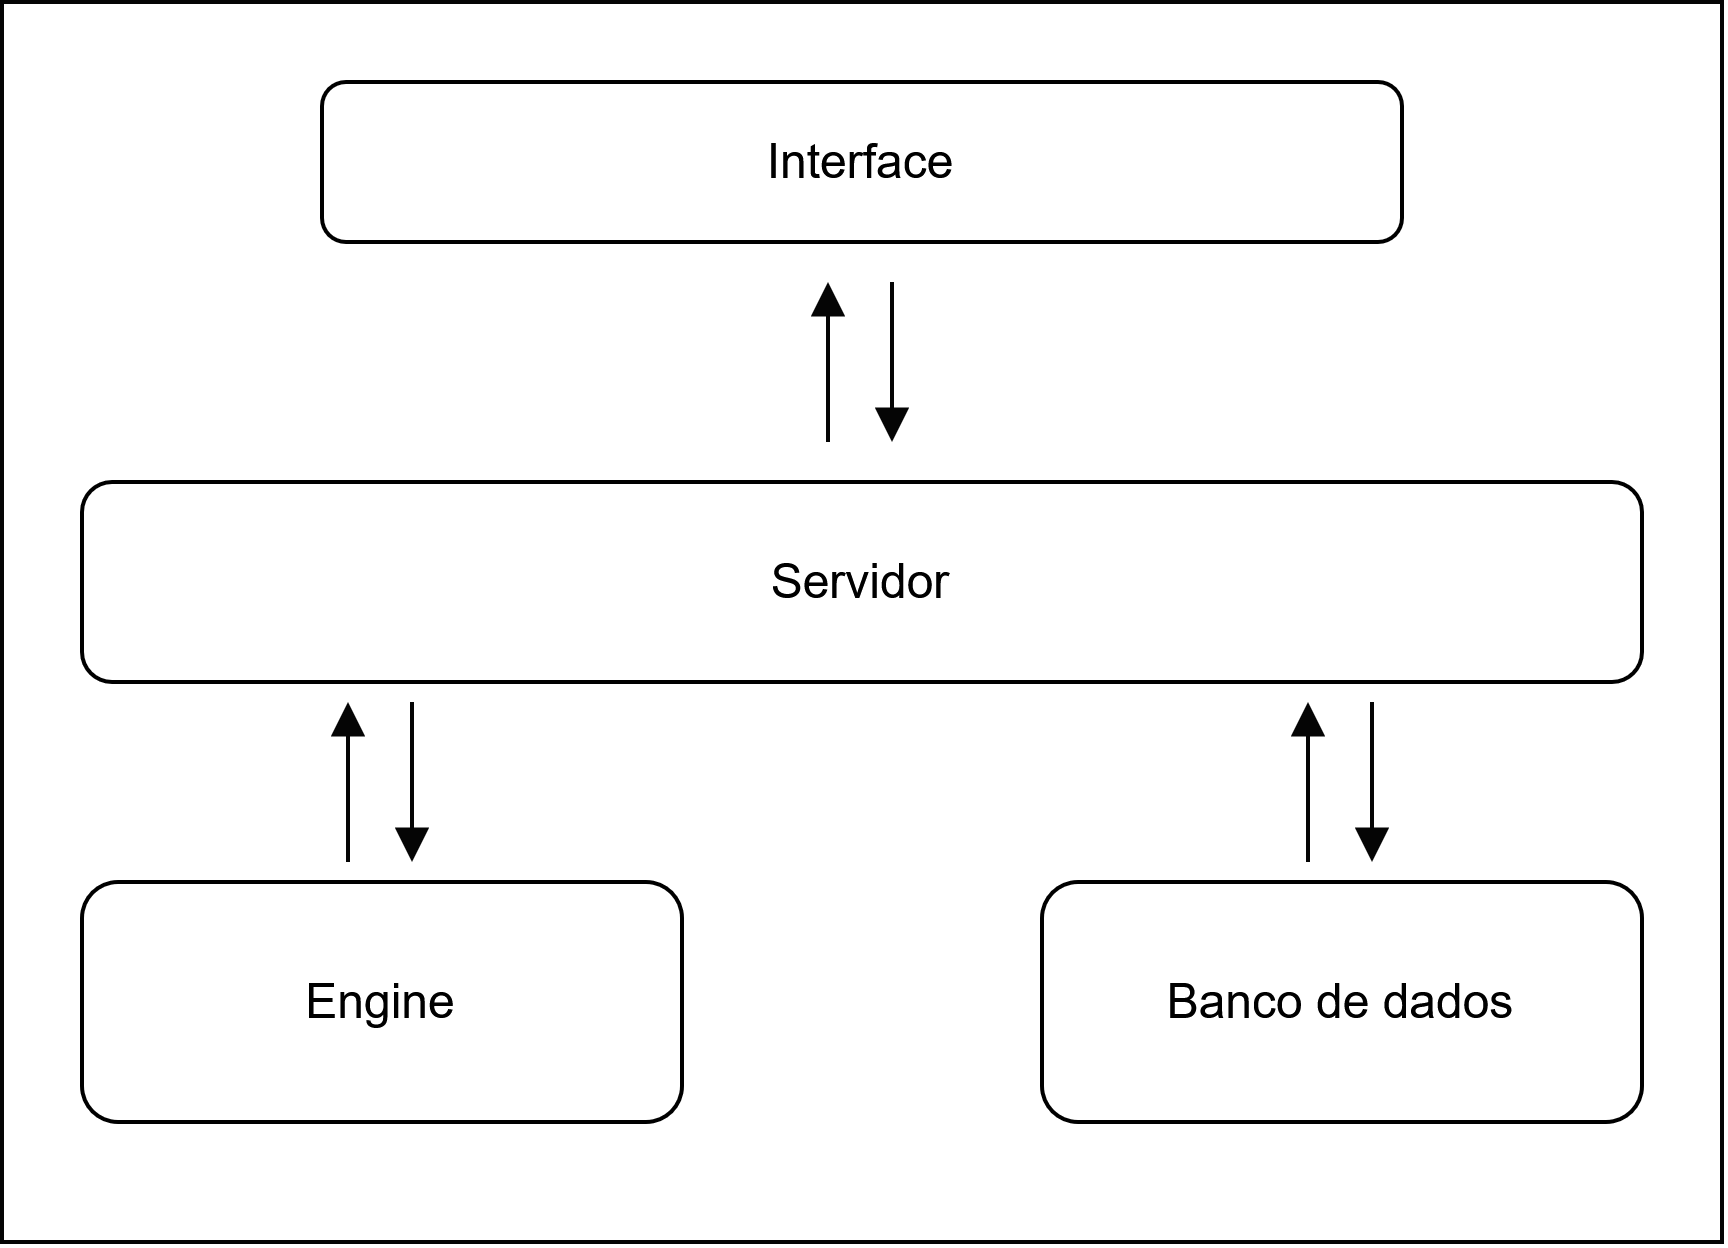
\includegraphics[width=0.9\linewidth]{images/system_overview.png}
        \caption{Visão geral do sistema}
        \label{fig:system_overview}
    \end{figure}

    \begin{figure}[H]
        \centering
        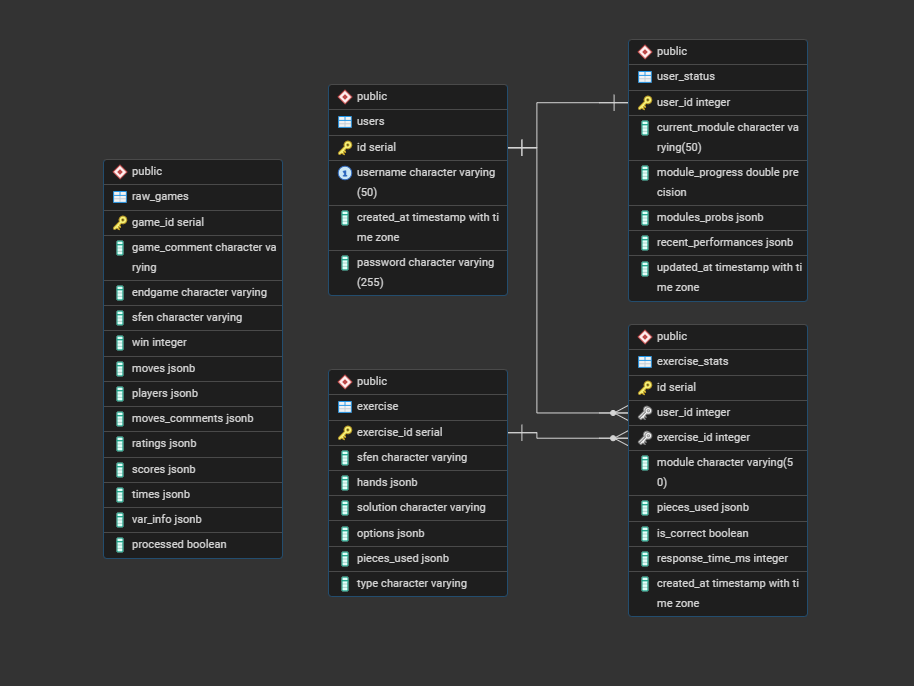
\includegraphics[width=0.9\linewidth]{images/tables.png}
        \caption{Tabelas do banco de dados}
        \label{fig:db_tables}
    \end{figure}
    
     \section{Banco de dados}
     \label{sec:database}
    O sistema utiliza o \textit{PostgreSQL} para armazenar informações dos usuários e dos exercícios. A escolha desse sistema foi motivada pela experiência prévia do autor com a ferramenta e pela facilidade de integração com Python por meio de bibliotecas como \textit{SQLAlchemy}, utilizada para definir modelos e realizar operações sobre os dados; \textit{psycopg}, responsável pela comunicação com o banco de dados; e \textit{Alembic}, empregado para gerenciar alterações no esquema do banco por meio de migrações. As tabelas são apresentadas na Figura~\ref{fig:db_tables} e são descritas abaixo:

    \begin{itemize}
        \item \textbf{raw\_games}: armazena os dados brutos de partidas extraídas da plataforma WDoor\textsuperscript{\cite{wdoor}}, que disponibiliza partidas no formato CSA, apresentado na seção~\ref{sec:server}.
        \item \textbf{users}: armazena os dados de cadastro dos usuários do sistema, incluindo o hash da senha, em vez da senha original.
        \item \textbf{user\_status}: contém informações referentes ao progresso do usuário. 
        \begin{itemize}
            \item \textbf{current\_module}: identifica o módulo em que o usuário se encontra.
            \item \textbf{module\_progress}: registra o progresso do usuário no módulo atual.
            \item \textbf{modules\_probs}: armazena a distribuição de probabilidades utilizada para orientar a recomendação dos módulos de exercícios.
            \item \textbf{recent\_performances}:  mantém um histórico do desempenho do usuário nos módulos.
        \end{itemize}
        \item \textbf{exercise}: contém os dados dos exercícios gerados.
        \begin{itemize}
            \item \textbf{sfen}: representação SFEN do estado do tabuleiro.
            \item \textbf{hands}: peças que cada jogador tem em mãos.
            \item \textbf{solution}: solução do exercício.
            \item \textbf{options}: alternativas do exercício, que incluem a solução.
            \item \textbf{pieces\_used}: peças utilizadas na solução do exercício.
            \item \textbf{type}: módulo ao qual o exercício pertence.
        \end{itemize}
        \item \textbf{exercise\_stats}: armazena as estatísticas das respostas enviadas pelos usuários para os exercícios.
        \begin{itemize}
            \item \textbf{user\_id}: identificação única do usuário.
            \item \textbf{exercise\_id}: identificação única do exercício.
            \item \textbf{module}: módulo ao qual o exercício pertence.
            \item \textbf{pieces\_used}: mesmo campo presente na tabela \textbf{exercise}.
            \item \textbf{is\_correct}:  indica se a resposta foi correta (True) ou incorreta (False).
            \item \textbf{response\_time}: tempo, em milissegundos, gasto pelo usuário para responder ao exercício.
        \end{itemize}
    \end{itemize}

    \section{\textit{Engine}}
    Assim como mencionado no início desta seção, o sistema utiliza a \textit{engine} YaneuraOu, baseada em um modelo NNUE (\textit{Efficiently Updatable Neural Network}). Escolheu-se essa \textit{engine} por não depender de uma placa de vídeo poderosa, o que viabilizou usá-la num ambiente local. Como a comunicação com o YaneuraOu ocorre através do envio de comandos USI pela entrada do próprio processo e lê-se a saída devolvida, optou-se por separá-lo do servidor. Assim, utilizou-se a biblioteca \textit{FastAPI} para criar um serviço que realiza a comunicação entre os dois processos, com o benefício do servidor não ser prejudicado quando a \textit{engine} apresentar algum erro.

    \begin{figure}[H]
        \centering
        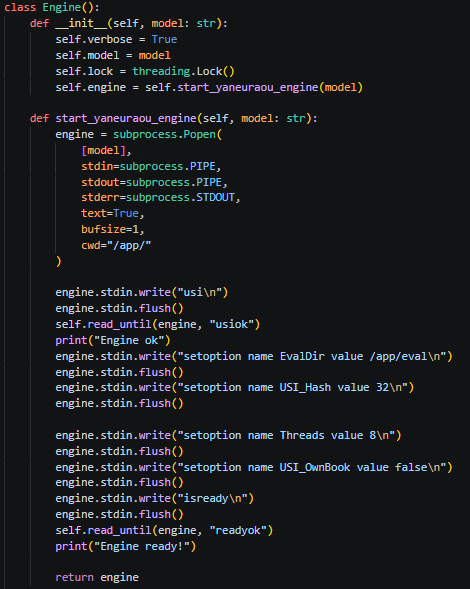
\includegraphics[width=0.9\linewidth]{images/engine_init.png}
        \caption{Inicialização da \textit{engine}}
        \label{fig:engine_init}
    \end{figure}

    Para inicializar o YaneuraOu, envia-se o comando \textit{usi}. Após ele enviar a mensagem \textit{usiok}, envia-se o comando 
    \textit{setoption name EvalDir value <path>}, onde \textit{path} se refere ao caminho para o diretório que contém os pesos da rede neural utilizada na avaliação das posições. Em seguida, são realizadas algumas configurações de desempenho. Por fim, envia-se o comando \textit{isready} e, após a \textit{engine} enviar \textit{readyok}, a inicialização está finalizada.
    
    Embora inicialmente estivesse previsto o uso do YaneuraOu na geração de exercícios de todos os módulos, durante o desenvolvimento verificou-se que ele seria necessário apenas no módulo de xeque-mate em um lance, no qual é empregado para auxiliar na geração de alternativas de resposta. O processo de geração dessas alternativas é apresentado na seção~\ref{sec:server}.
    
    \section{Servidor}
    \label{sec:server}
    Para o desenvolvimento do servidor, utilizou-se a biblioteca \textit{FastAPI}, responsável pela criação e pelo gerenciamento dos endpoints da API consumida pela interface do sistema. Esse componente ficou responsável pelas seguintes funcionalidades:
    
    \begin{itemize}
    \item Gerar os exercícios automaticamente;
    \item Organizar os exercícios em listas;
    \item Corrigir os exercícios e gerar a explicação;
    \item Realizar o cadastro e a autenticação dos usuários;
    \item Atualizar e consultar as estatísticas de desempenho dos usuários;
    \item Gerenciar a comunicação com o banco de dados.
    \end{itemize}

    \subsection{Arquitetura}
    O servidor utiliza uma arquitetura em camadas, com o objetivo de separar as responsabilidades dos componentes do sistema, facilitando sua manutenção e isolando a implementação de cada funcionalidade. Dessa forma, o código foi organizado em três camadas:
    \begin{itemize}
        \item Repositórios: responsáveis por realizar as operações de persistência e consulta de dados no banco de dados.
        \item Serviços:  responsáveis por implementar e gerenciar a lógica de funcionamento do sistema.
        \item Roteadores: responsáveis por definir os endpoints da API, recebendo as requisições dos clientes e encaminhando-as aos serviços correspondentes.
    \end{itemize}

    Durante o processamento de uma requisição, o roteador aciona o serviço responsável pela funcionalidade solicitada, que, quando necessário, utiliza os repositórios para acessar o banco de dados. O fluxo é representado na Figura~\ref{fig:server_architecture}.

    \begin{figure}[H]
        \centering
        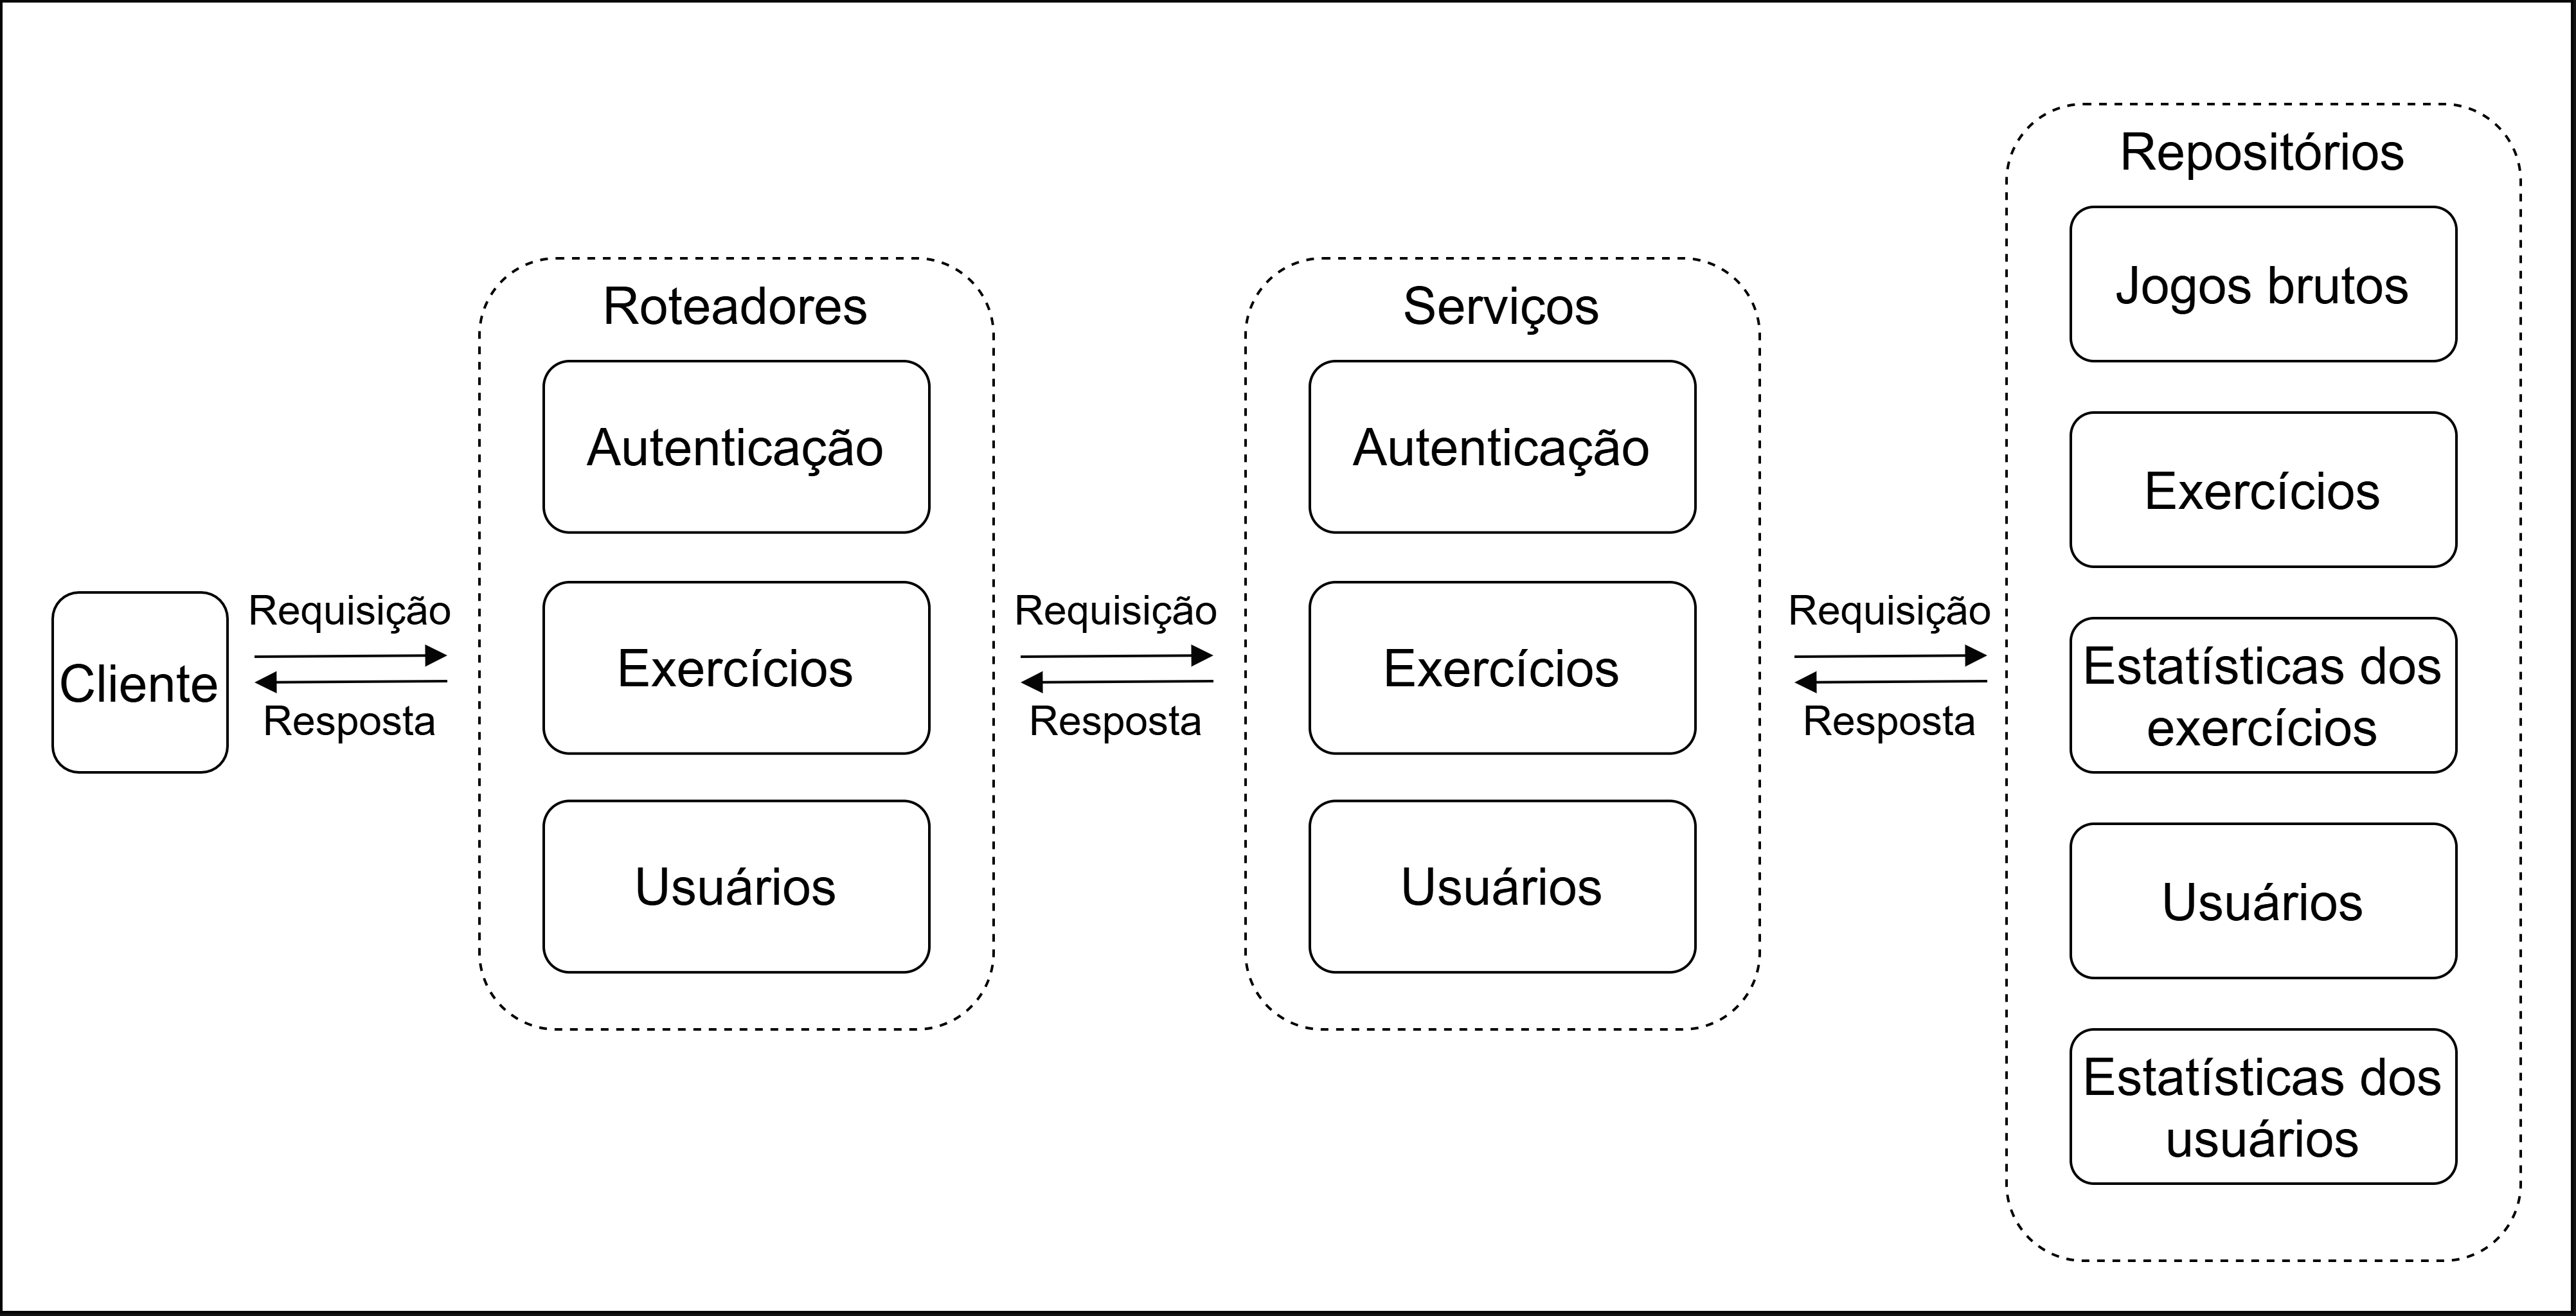
\includegraphics[width=1.0\linewidth]{images/server_architecture.png}
        \caption{Arquitetura do servidor}
        \label{fig:server_architecture}
    \end{figure}
    
    Além dessas camadas, foram utilizados esquemas do Pydantic para estruturar e validar os dados recebidos e retornados pelos endpoints, garantindo um formato padronizado para a comunicação entre o cliente e o servidor.


    \subsection{Geração automática de exercícios}
    Para padronizar a apresentação dos exercícios e simplificar a sua implementação na interface, todas as questões consideram que é a vez do jogador \textit{sente} de jogar.
    Cada questão apresenta quatro alternativas, das quais apenas uma é a correta, e pertence a um dos seguintes módulos:
    \begin{itemize}
        \item \textbf{Reconhecimento}: pede para que o usuário identifique uma determinada peça no tabuleiro.
        \item \textbf{Movimento 1}: apresenta apenas uma peça sem o símbolo escrito no tabuleiro com seus movimentos destacados e pede para que o usuário identifique qual seria tal peça.
        \item \textbf{Movimento 2}: semelhante ao Movimento 1, mas existem outras peças no tabuleiro que impedem alguns movimentos.
        \item \textbf{Promoção}: pede para que o usuário identifique qual movimento pode levar a uma promoção. 
        \item \textbf{Drop}: pede para que o usuário identifique qual movimento constitui um \textit{drop} legal.
        \item \textbf{Xeque-mate}: pede para que o usuário identifique qual movimento leva ao xeque-mate.
    \end{itemize}

    Assim como mencionado na seção~\ref{sec:database}, os exercícios são gerados a partir de uma plataforma que contém partidas entre jogadores reais, com o intuito de garantir que as posições apresentadas no tabuleiro são legais e expor os usuários do sistema a cenários encontrados em partidas reais. Esses jogos são disponibilizados no formato CSA, arquivos que contêm informações como nome dos jogadores, registro dos movimentos, estado do tabuleiro ao final da partida no formato SFEN e qual foi o vencedor.
    Para processar os dados dos jogos, foi utilizada uma biblioteca chamada \textit{cshogi}\textsuperscript{\cite{cshogi}}, que permite manipular um tabuleiro de shogi, extrair informações, como a posição das peças e as mãos de cada jogador a partir da representação SFEN, simular movimentos e verificar a legalidade das jogadas. Dessa forma, para cada jogo, a geração segue os passos abaixo:

    \begin{enumerate}
        \item Simulação dos movimentos registrados;
        \item Para cada movimento, são definidas a solução e as opções de acordo com os critérios de cada módulo.
        \item Registro desse exercício em uma lista para o posterior registro no banco de dados.
    \end{enumerate}

    Mais detalhes do passo 2 estão descritos abaixo:

    \begin{itemize}
        \item \textbf{Reconhecimento}:
        A solução consiste em selecionar aleatoriamente uma peça no tabuleiro. As alternativas são compostas pela solução e outras três peças diferentes. Por exemplo, se um peão é escolhido como solução, as outras alternativas podem ser lança, cavalo e rei.
        \item \textbf{Movimento 1}: Nesse módulo, não é necessário utilizar os jogos extraídos da plataforma. Para cada uma das 14 peças possíveis, é definido um tabuleiro que contém apenas essa peça em sua região central, representado pelo SFEN 9/9/9/9/<peça>/ 9/9/9/9. Em seguida, as alternativas são selecionadas entre as peças restantes que apresentam padrões de movimento diferentes do padrão da solução, evitando a possibilidade de mais de uma resposta correta. Por exemplo, caso a solução seja um general de ouro, as alternativas não poderão incluir peças promovidas, com exceção da torre e do bispo promovidos, pois as demais possuem o mesmo padrão de movimento do general de ouro.
        \item \textbf{Movimento 2}: Diferentemente do módulo Movimento 1, uma peça presente no tabuleiro de uma partida real é selecionada aleatoriamente para ser a solução. As alternativas são determinadas seguindo o mesmo critério do módulo anterior. Entretanto, a presença de outras peças no tabuleiro pode restringir os movimentos disponíveis, adicionando uma camada de dificuldade, pois nem todos os movimentos possíveis de uma peça estarão necessariamente disponíveis na posição apresentada.  
        \item \textbf{Promoção}: Inicialmente, é selecionado aleatoriamente um movimento que permite a promoção de uma peça. Durante a seleção das alternativas, são descartados os movimentos que também resultariam na promoção de uma peça. Além disso, para cada movimento de promoção descartado, também é eliminado o movimento correspondente sem promoção, mesmo que nenhum dos dois corresponda à solução. Isso evita que duas alternativas representem a mesma jogada, diferenciando-se apenas pela decisão de promover ou não a peça. Por exemplo, se a solução for 8d->8c+ e uma das alternativas possíveis for 7d->7c+, esta última será descartada, assim como 7d->7c.
        \item \textbf{Drop}: O processo é semelhante ao módulo Promoção. Um movimento de drop é escolhido aleatoriamente e definido como a solução do exercício. Em seguida, os demais movimentos de drop legais são descartados. Por fim, as alternativas são constituídas por movimentos de drop ilegais, como o posicionamento de um peão em uma coluna que já contém outro peão aliado.
        \item \textbf{Xeque-mate}: Verifica-se se determinado movimento resulta em xeque-mate. Caso isso ocorra, o movimento identificado e o estado do tabuleiro são enviados para a \textit{engine}, responsável pela geração das alternativas. Seu uso nesse processo permite selecionar movimentos candidatos com base na posição, tornando as alternativas mais plausíveis e, consequentemente, aumentando a dificuldade do exercício. Isso evita que movimentos claramente distantes da região onde se encontra o rei adversário evidenciem facilmente a resposta correta. Por exemplo, suponha que a solução seja mover um general de ouro da casa 4d para a casa 5c. Caso as alternativas incluam movimentos de peões para casas distantes do rei adversário, como as linhas g ou h, torna-se mais fácil identificar a solução. No entanto, é possível que dentre os movimentos escolhidos pelo YaneuraOu, exista mais de um xeque-mate. Dessa forma, esses movimentos são também excluídos.
        
    \end{itemize}